\renewcommand{\headrulewidth}{1pt}
\fancyhead[C]{\textbf{Entraînement -- Calcul littéral niveau 1 version \no <<version>>}} 
\fancyhead[L]{}
\fancyhead[R]{Cycle 4}

\renewcommand{\footrulewidth}{1pt}
\fancyfoot[C]{} 
\fancyfoot[L]{}
\fancyfoot[R]{Calcul littéral niveau 1}

\subsection*{Objectifs de cette fiche :}
{\setlength{\multicolsep}{0cm}
\setlength{\columnsep}{.2cm}
\setlength{\columnseprule}{0pt}
\vspace{0cm}
	\begin{multicols}{2}
		\begin{itemize}
			\renewcommand{\labelitemi}{\SquareCastShadowBottomRight}
			\item Produire une expression littérale.
			\item Calculer la valeur d'une expression littérale (pour un nombre positif).
			\item Simplifier et réduire une expression littérale.
			\item Développement simple
		\end{itemize}
	\end{multicols}
}

\begin{methode}[frametitle=Méthodes]
\begin{itemize}
	\item \textbf{Pour calculer la valeur d'une expression littérale}, on remplace les lettres par les valeurs données et on écrit les $\times$ sous-entendus (devant une lettre ou une parenthèse)
	
	\item \textbf{Pour développer une expression}, on utilise la distributivité de la multiplication sur l'addition : $\mathbf{k(a+b)=ka+kb}$.
	
	\item \textbf{Pour réduire une expression}, on regroupe tous les termes semblables.	
\end{itemize}

\end{methode}



\begin{multicols}{2}

% Il faudrait créer une variable python ["le double","le triple","le quadruple","le quintuple","la moitié",le "tiers","le quart", "le cinquième", "le dixième"] et l'utiliser dans l'exercice ainsi qu'une variable ["la somme", "la différence", "le produit", "le quotient"]
%\exo{}
%
%Traduire par une expression littérale : 
%\begin{enumerate}
%	\item le double de $z$
%	\item le triple de $z$
%	\item la moitié de $z$
%	\item le produit de 7 par $z$
%	\item la somme du produit de 5 par $z$ et du\\ double de $z$
%	\item le double de la somme de 5 et $z$
%\end{enumerate}

\exo{}
Quel résultat donne chacun de ces 3 programmes de calculs lorsqu'on prend $x$ comme nombre de départ ?	

\begin{center}
\fcolorbox{black}{gray!30}{
\begin{minipage}{0.7\linewidth}
Programme 1 : 
\begin{itemize}
	\item Multiplier par <<nZ[1]>>
	\item Ajouter <<nZ[2]>>
\end{itemize}
\end{minipage}
}

\medskip
\fcolorbox{black}{gray!30}{
\begin{minipage}{0.7\linewidth}
Programme 2 : 
\begin{itemize}
	\item Soustraire <<nZ[3]>>
	\item Multiplier par <<nZ[4]>>
\end{itemize}
\end{minipage}
}


\medskip
\fcolorbox{black}{gray!30}{
\begin{minipage}{0.7\linewidth}
Programme 3 : 
\begin{itemize}
	\item Multiplier par <<nZ[5]>>
	\item Soustraire <<nZ[6]>>
	\item Prendre le double
\end{itemize}
\end{minipage}
}

\end{center}


\exo{}

Simplifier les expressions suivantes.

\begin{multicols}{2}
$A=x <<terme(S[1])>> x$\\
$B=<<S[2]>>x\times x$\\
$C=<<nZ[7]>>\times x <<terme(nZ[8])>>\times x$\\
$D=<<nZ[7]>>\times x\times <<facteur(nZ[8])>>\times x$\\
$E=<<nZ[9]>> \times x<<terme(nZ[10])>>\times <<facteur(nZ[11])>> <<terme(nZ[12])>> x$\\
$F=<<nZ[13]>> \times (y\times <<facteur(nZ[14])>> <<terme(nZ[15])>> \times <<facteur(nZ[16])>>)$\\
$G=<<N2[1]>> a\times  a+a\times <<N2[2]>>+a\times <<N3[1]>>$\\
$H= <<nZ[17]>>\times x <<terme(nZ[18])>>$
\end{multicols}



\exo{}

Calculer les expressions suivantes pour $x=<<n[19]>>$.

\begin{tasks}[counter-format = {tsk[1].},label-format={\bfseries}](3)
	\task $<<n[20]>> x$ 
	\task $x^2$
	\task $<<n[21]>>x <<terme(n[22])>> $
	\task $ <<n[23]>> (<<nZ[24]>> x <<terme(nZ[25])>>)$
	\task $ <<n[26]>>  <<terme(nZ[27])>> x$
	\task $x^3$
\end{tasks}

\exo{}

Développer les expressions suivantes.

\begin{multicols}{2}
$A=  <<nZ[28]>> (x  <<terme(nZ[29])>>)$\\
$B= <<nZ[30]>> ( <<nZ[31]>> x    <<terme(nZ[32])>>)$\\
$C=y( <<nZ[33]>>  <<terme(nZ[34])>> y)$\\
$D= <<nZ[35]>>  t(  <<nZ[36]>> t <<terme(nZ[37])>>)$
\end{multicols}







\raggedcolumns
\end{multicols}

\exon{}

\begin{minipage}{0.4\linewidth}
	\begin{center}
	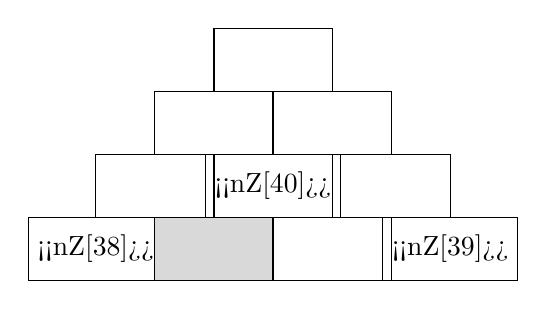
\begin{tikzpicture}
		\tikzstyle{brique}=[minimum width=1.5cm, minimum height=0.8cm,draw]
		\tikzstyle{brique_grise}=[minimum width=1.5cm, minimum height=0.8cm,draw,fill=gray!30]
		\node[brique] at (0,0) {  <<nZ[38]>> }; % gauche
		\node[brique_grise] at (1.5,0) {};
		\node[brique] at (3,0) {};
		\node[brique] at (4.5,0) { <<nZ[39]>> };  % droite
		\node[brique] at (.75,.8) {};
		\node[brique] at (2.25,.8) {  <<nZ[40]>> };  % milieu bas
		\node[brique] at (3.75,.8) {};
		\node[brique] at (1.5,1.6) {};
		\node[brique] at (3,1.6) {};
		\node[brique] at (2.25,2.4) {};
	\end{tikzpicture} 	
\end{center}
\end{minipage}
\begin{minipage}{0.6\linewidth}
Pour compléter cette pyramide, le nombre situé dans une case est la somme des deux nombres situés en dessous de lui.

\begin{enumerate}
	\item Compléter cette pyramide en mettant un nombre au choix dans la case grise.
	\item Benjamin affirme : \og{} Quel que soit le nombre que je place dans la case grise, je trouve toujours <<nZ[38] + nZ[39] + 2*nZ[40]>> dans la case la plus haute. \fg{}. Est-ce vrai ou faux ? Démontrer le.
\end{enumerate}
\end{minipage}


%\exon{}
%
%
%\begin{center}
%\fcolorbox{black}{gray!30}{
%\begin{minipage}{0.5\linewidth}
%\begin{itemize}
%	\item Multiplier par <<nZ[41]>>
%	\item Enlever <<nZ[41]>>
%	\item Multiplier par <<nZ[41]>>
%	\item Ajouter <<nZ[41]>>
%	\item Enlever quatre fois le nombre de départ
%\end{itemize}
%\end{minipage}
%}
%\end{center}
%
%\begin{enumerate}
%	\item Après avoir lu ce programme, Benjamin dit : \og{} C'est complètement inutile de faire toutes ces étapes, en un seul calcul je trouve le résultat. \fg{}.\\
%Démontrer que Benjamin a raison et expliquer la seule étape nécessaire.
%	\item Quel nombre de départ faut-il choisir pour obtenir 13 comme résultat avec ce programme de calcul ?
%\end{enumerate}
%
%\exon{}
%
%\begin{tabularx}{\linewidth}{*{4}{>{\centering\arraybackslash}X}}
%\begin{tikzpicture}
%	\tikzstyle{carré}=[minimum width=.5cm, minimum height=.5cm,draw]
%	\node[carré] at (0,0) {};
%\end{tikzpicture}
%&
%\begin{tikzpicture}
%	\tikzstyle{carré}=[minimum width=.5cm, minimum height=.5cm,draw]
%	\node[carré] at (0,0) {};
%	\node[carré] at (-.5,0) {};
%	\node[carré] at (.5,0) {};
%	\node[carré] at (0,.5) {};
%\end{tikzpicture}
%&
%\begin{tikzpicture}
%	\tikzstyle{carré}=[minimum width=.5cm, minimum height=.5cm,draw]
%	\node[carré] at (0,0) {};
%	\node[carré] at (-.5,0) {};
%	\node[carré] at (-1,0) {};
%	\node[carré] at (.5,0) {};
%	\node[carré] at (1,0) {};
%	\node[carré] at (0,.5) {};
%	\node[carré] at (0,1) {};
%\end{tikzpicture}
%&
%\begin{tikzpicture}
%	\tikzstyle{carré}=[minimum width=.5cm, minimum height=.5cm,draw]
%	\node[carré] at (0,0) {};
%	\node[carré] at (-.5,0) {};
%	\node[carré] at (-1,0) {};
%	\node[carré] at (-1.5,0) {};
%	\node[carré] at (.5,0) {};
%	\node[carré] at (1,0) {};
%	\node[carré] at (1.5,0) {};
%	\node[carré] at (0,.5) {};
%	\node[carré] at (0,1) {};
%	\node[carré] at (0,1.5) {};
%\end{tikzpicture}
%\\[-.1cm]
%\textbf{Étape 1} & \textbf{Étape 2} & \textbf{Étape 3} & \textbf{Étape 4}\\
%\end{tabularx}
%
%\bigskip
%\begin{enumerate}
%    \item Combien faut-il de carrés à l'étape 5 ?
%    \item Proposer une formule permettant de calculer le nombre de
%      carrés nécessaires pour l'étape $N$.
%    \item Combien faut-il de carrés à l'étape 1~000 ?
%\end{enumerate}


	